\part{Fluid Simulation}
\begin{multicols}{2}
\section{Spatial Discretization}
There are two common spatial discretizations:
\begin{itemize}
	\item \emph{Langragian} viewpoint
		\begin{itemize}
			\item Particles can move freely in space and carry quantities,
			\item Fluid motion is described by moving particles around.
			\begin{figure}[H]
				\centering
				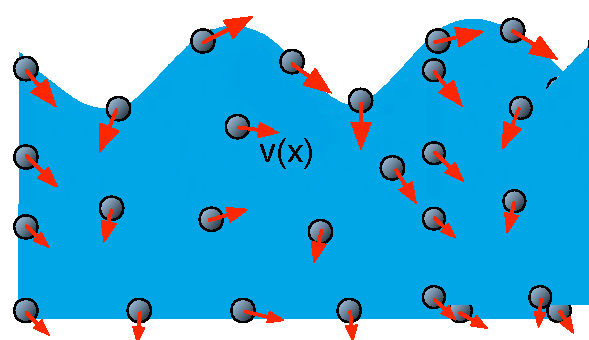
\includegraphics[width=0.35\textwidth,page=1]{img/05_spatial_discretization}
			\end{figure}
			Features
			\begin{description}
				\item[/] \emph{Incompressibility}
				\item[+] \emph{Complex interactions}
				\item[+] \emph{Splashes, droplets}
				\item[+] \emph{Advection}
				\item[-] \emph{Smooth Surfaces}
			
			\end{description}
		\end{itemize}
	\item \emph{Eulerian} viewpoint
		\begin{itemize}
			\item Fixed spatial locations
			\item Measure quantities as it flows past
		\end{itemize}
		\begin{figure}[H]
				\centering
				\includegraphics[width=0.3\textwidth,page=2]{img/05_spatial_discretization}
			\end{figure}
			Features
			\begin{description}
				\item[+] \emph{Incompressibility}
				\item[/] \emph{Complex interactions}
				\item[-] \emph{Splashes, droplets}
				\item[-] \emph{Advection}
				\item[+] \emph{Smooth Surfaces}
			
			\end{description}
\end{itemize}
\subsection{Notation}
	\begin{align*}
		\text{Gradient: }\nabla u &= \begin{pmatrix}
 										u_x \\ u_y \\ u_z
 									  \end{pmatrix}\\
		\text{Divergence: }\nabla \cdot u &= u_x + u_y + u_z\\
		\Delta u &= \nabla^2 u = \nabla \cdot \nabla u = u_{xx} + u_{yy} + u_{zz}
	\end{align*}


\subsection{Navier-Stokes Equations}
The \emph{Navier-Stokes Equations} are 2 differential equations describing a velocity field over time.\\

Symbols:
\begin{align*}
 u &= \text{ velocity}\\
 p &= \text{ pressure}\\
 \rho &= \text{ density}\\
 g &= \text{ gravity}\\
 \nu &= \text{ viscosity (kinematic)}
\end{align*}

\begin{description}
	\item[Conservation of momentum]
		\begin{align*}
			\underbrace{{\partial u \over \partial t} + (u \cdot \nabla) u}_\text{advection}
				&= 
			\underbrace{-{1\over \rho}\nabla p}_\text{pressure} +
			\underbrace{\nu \Delta u}_\text{viscosity} + g
		\end{align*}
		Consider a single blob of fluid $p$. Which has mass $m$, volume $V$ and velocity $u$. We start with Netwon's  second law $F = ma$ and rewrite it as $F =  m {Du \over Dt}$.\\
		
		\emph{Forces acting on the fluid}
		\begin{itemize}
			\item \emph{Gravity}: $mg$
			\item \emph{Pressure}: The surrounding has to be considered. The particle experiences a negative gradient towards the largest pressure decrease (low pressure areas)
			Computed with 
			\begin{align*}
				-\nabla p\ V
			\end{align*}
			\item \emph{Viscosity}: Can be described as "internal friction" and more accurately as \emph{diffusion of velocities}.
			\item \emph{Diffusion} Strength of dynamic viscosity coefficient:
				\begin{align*}
					V \mu \nabla \cdot \nabla u &= V \mu \Delta u
				\end{align*}
		\end{itemize}
		Deduction of formula:
		\begin{align*}
			\text{Newton's second law:} \ \ F &= ma\\
			F &= m {Du \over Dt}\\
			mg - V\nabla p +  V\mu\Delta u &= m{Du \over Dt} &\text{Forces so far}\\
			\rho g - \nabla p + \mu \Delta u &= \rho {Du\over Dt}& \text{Divide by $V$}\\
			g - {1 \over \rho} \nabla p + {\mu \over \rho} \Delta u &= {Du \over Dt} &\text{Divide by Density}
		\end{align*}
		Rearrange and use kinematic viscosity:
		\begin{align*}
			{Du \over Dt} &= - {1\over \rho} \nabla p + \nu \Delta u + g
		\end{align*}
		The viscosity term is usually left out on grid based simulations since inaccuracies are introduced. \emph{Particle simulations} need viscosity to stabilise the system!
	\item[Material Derivative] Change of a quantity $q(t,x)$ during motion:
		\begin{align*}
			{d\over dt} q(t, x) &= {\partial q\over \partial t} + {\partial q \over \partial x} \cdot {d x\over dt}\\
			&= \underbrace{{\partial q \over  \partial t}}_\text{change of $q$ at fixed point} + \underbrace{\nabla q \cdot u}_\text{in-/outflow}\\
			&= {Dq \over  Dt}
		\end{align*}
		The material derivative result in two different viewpoints:
			\begin{itemize}
				\item \textbf{Eulerian viewpoint}: Use both the change of $q(t,x)$ and the in-/outflow:
					\begin{align*}
						{Dq \over  Dt} &= {\partial q \over  \partial t} + {\nabla q \cdot u}
					\end{align*}
				\item \textbf{Lagrangian viewpoint}: Only the change of $q(t,x)$ is used:
					\begin{align*}
						{Dq \over  Dt} &= {\partial q \over  \partial t} + {\nabla q \cdot u}
					\end{align*}

			\end{itemize}
 

	\item[Conservation of mass] 
		\begin{align*}
			\nabla \cdot u &= 0
		\end{align*}
		This condition also models \emph{incompressibility}.\\
		
		Reformulating the equation
		\begin{align*}
			\text{We have:}\quad \nabla \cdot u &= 0\\
				u'^{n} &= f(u^n)\\
				u^{n+1} &= u'^n -\Delta t {1\over \rho} \nabla p\\
			\text{Thus:}\quad \nabla \cdot u^{n+1} &= 0\\
			\text{Insert:}\quad \nabla \cdot u'^n -\Delta t {1\over \rho} \nabla \cdot \nabla p &= 0\\
			\text{Reaarange:}\quad \nabla \cdot \nabla \cdot p &= {\rho \over \Delta t} \nabla \cdot u'^n
		\end{align*}
		Results in a \emph{Poisson Equation} since the right side of the equation is fully known.
		
\end{description}

\subsection{Numerical Solution}
\begin{description}
	\item[Time discretisation] with fixed time step $\Delta t$
		\begin{figure}[H]
			\centering
			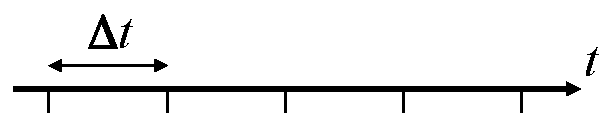
\includegraphics[page=1,width=0.35\textwidth]{img/05_discretisation}
		\end{figure}
	\item[Space discretisation] Use a staggered grid (\emph{MAC grid}) with cubical cells. The velocity components are defined on the faces of the cells (so that the staggering is more stable). The pressure is defined at the center of the grid.
		\begin{figure}[H]
			\centering
			\includegraphics[page=2,width=0.35\textwidth]{img/05_discretisation}
		\end{figure}
\end{description}

\subsubsection{Central Differences}
Central differences provide an accuracy of $\bigO{(\Delta x)^2}$:
\begin{align*}
	{\partial q \over \partial x} &= {q_{i+1} - q_{i-1} \over 2 \Delta x}
\end{align*}
The computation can run into a null space problem since not only the constant function evaluates to zero.
Solutions:
\begin{itemize}
	\item Use forward or backward difference
	\item Make use of staggered grid and and sample $q$ qt half-way points:
		\begin{align*}
			{\partial q \over \partial x} &= {q_{i+1/2} - q_{i-1/2} \over \Delta x}
		\end{align*}

\end{itemize}
%\subsubsection{Solution Overview}
%Use conservation of momentum to update velocity field:
%\begin{enumerate}
%	\item Advect velocities with themselves. Solve:
%		\begin{align*}
%			{\partial u \over \partial t} + (u \cdot \nabla) u
%		\end{align*}
%
%	\item Add external forces
%	\item Choose pressure so that velocity field is divergence free (ensure conservation of mass).
%\end{enumerate}

\subsubsection{Algorithm Summary}
\begin{enumerate}
	\item Update grid (mark cells)
	\item Advance the velocity field:
		\begin{itemize}
			\item Advection (semi-Lagrange step for each velocity component)
			\item Apply external forces (gravity,...)
			\item Calculate and apply pressure (divergence-free) 
		\end{itemize}
	\item Move marker particles
	\item Start over...
\end{enumerate}

\section{SPH Solvers}
Instead of solving the \emph{Navier-Stokes equations} on a grid, we are using particles instead. SPH solvers are therefore Langrangian based solvers. 
Each particle represents a volume. This assumes that fluids are continuous: \emph{Continuum assumption}
\begin{itemize}
	\item Properties such as density, pressure, velocity, etc are well-defined at "infinitely" many points.
	\item Properties are assumed to \emph{vary continuously} from one point to another.
\end{itemize}
Equations for the particle method:
		\begin{align*}
			\underbrace{{\partial u \over \partial t}}_\text{advection}
				&= 
			\underbrace{-{1\over \rho}\nabla p}_\text{pressure} +
			\underbrace{\nu \Delta u}_\text{viscosity} + g\\
			\nabla \cdot u &= 0
		\end{align*}
\begin{itemize}
	\item The total mass is conserved as long as the particle number is \emph{constant}. This however doesn't imply that the fluid is incompressible.
	\item The velocity divergence $\neq 0$: Therefore the density varies inside the fluid.
\end{itemize}

\subsection{SPH}
Particles concentrate mass at a point. A continuos field is described by smooth particles: A smoothing kernel describes distribution of attributes around particle:
\begin{figure}[H]
	\centering
	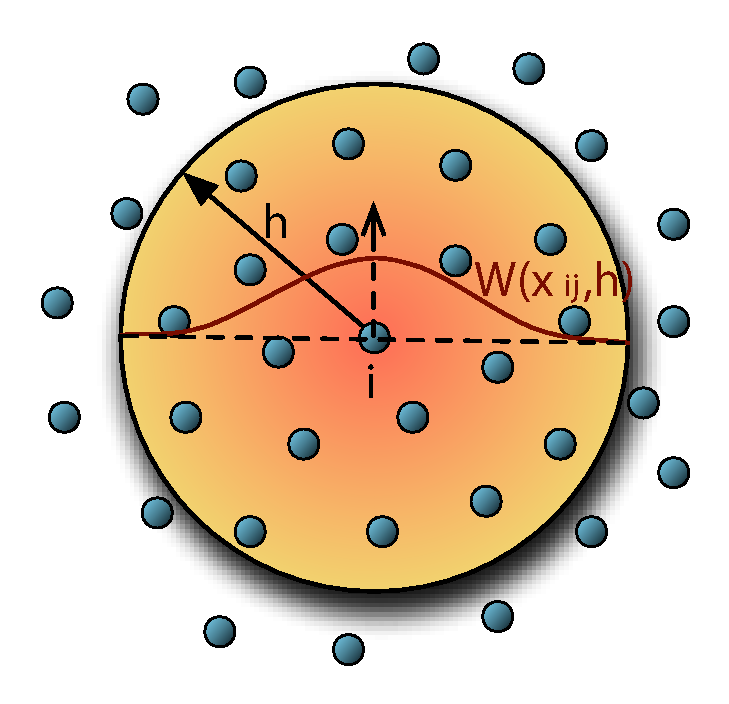
\includegraphics[width=0.35\textwidth]{img/05_sph}
\end{figure}

\subsubsection{Smoothing Kernels for SPH}
Each kernel is described by a integral representation of a field variable:
\begin{align*}
	A(x) &= \int_\Omega A(x)\delta(x-x')dx
\end{align*}
The dirac delta function is usually replaced by a smoothing kernel $W(x,h)$:
\begin{align*}
		A(x) &= \int_\Omega A(x)W(x-x', h)dx
\end{align*}
\emph{Kernel properties}
\begin{itemize}
	\item \emph{Normalisation condition}
		\begin{align*}
			\int W(x-x',h) dx' = 1
		\end{align*}
	\item \emph{Dirac delta function}
		\begin{align*}
			\lim_{h\mapsto 0} W(x-x', h) = \delta (x-x')
		\end{align*}
	\item \emph{Compact condition}
		\begin{align*}
			W(x-x', h) &= 0 \quad \text{when }\norm{x-x'} > h 
		\end{align*}
\end{itemize}

Several Kernels exist [Müller03], [Monaghang92,05]:
\begin{align*}
	W_{poly6} (x_{ij}, h) &= {315\over 64\pi h^9} 
			\begin{cases}
				(h^2-x_{ij}^2)^3 & 0\leq x_{ij} \leq h\\
				0 & \text{otherwise}
			\end{cases}\\
	W_{spiky} (x_{ij}, h) &= {15\over\pi h^6} 
			\begin{cases}
				(h-x_{ij})^3 & 0\leq x_{ij} \leq h\\
				0 & \text{otherwise}
			\end{cases}\\
	W_{viscous} (x_{ij}, h) &= {15\over 2\pi h^3} 
			\begin{cases}
				-{x_{ij}^3 \over 2h^3} + {x_{ij}^2 \over h^2} + {h\over 2x_{ij}}-1
					 & 0\leq x_{ij} \leq h\\
				0 & \text{otherwise}
			\end{cases}
\end{align*}

The smoothing can be computed like this for a location $A(x)$:
\begin{align*}
	 A(x) &= \sum_j {m_j\over \rho_j} A_j W(x-x_j, h).
\end{align*}
This is beneficial for the computation since the differentiation only affects the kernel. The gradient and laplacian can be easily calculated:
\begin{align*}
	 \nabla A(x) &= \sum_j {m_j\over \rho_j} A_j \nabla W(x-x_j, h)\\
	 \nabla^2 A(x) &= \sum_j {m_j\over \rho_j} A_j \nabla^2 W(x-x_j, h)\\
\end{align*}
\subsection{Density}
Each particle has the same mass $m$. The density field induced by a particle $i$ is:
\begin{align*}
	\rho_i &= \sum m_j W(x_{ij},h).
\end{align*}
Problem: The \emph{density is underestimated at the boundaries}. \\

Densities are initially set and evolve over time. This results in inaccuracies in a long-term simulation and thus make said simulation unstable.
Rate of change:
\begin{align*}
	{d \rho_i \over dt} &= \sum_j m_j (v_i - v_j) \cdot \nabla W(x_{ij}, h)
\end{align*}

\subsection{Pressure}
The density is used to compute the pressure of each particle. \emph{Equation of state} [Batchelor]:
\begin{align*}
	p_i &= {k\rho_0 \over \gamma} \left(\left( {\rho_i \over \rho_0 }\right)^\gamma - 1 \right)\\
	\rho_0 &: \text{ rest density of water ($1000 kg/m^3$)}\\
	k &: \text{ gas constant}\\
	\gamma &: \ 7
\end{align*}

\subsection{Pressure Force} 
The pressure density yields:
\begin{align*}
 F_i^{pressure} &= - {m_i \over \rho_i} \sum_j {m_j\over \rho_j} {p_i + p_j \over 2} \nabla W(x_{ij}, h)\\
&= - \sum_j {m_i m_j}\left( {p_i\over \rho_i^2} + {p_j \over \rho_j^2} \right) \nabla W(x_{ij}, h)\\
\end{align*}

\subsection{Time Stepping}
The time step size direrectly correlates with efficiency. In order to achieve $25$ fps we need to represent $0.04s$ per frame. With a $\Delta t=0.001$ we therefore need to compute $40$ simulation steps per frame. 

\subsubsection{Courant Condition}
If a particle is to be propagated with a maximum velocity $v$, it must not be integrated with a too large time step, or some grid points will be leaped. 
\begin{itemize}
	\item Each particle must not be passed by
		\begin{align*}
			\Delta t_c \leq \alpha {h\over c}
		\end{align*}
		where $c$ is for our case considered as the \emph{square root of the speed of sound}.
	\item High viscosity has to be considered as well (speed of sound is lower)
	\item \emph{Large forces} lead to 
		\begin{align*}
			\Delta t_f = 0.25 \cdot \min_i \left( {h\over \norm{f_i} } \right)
		\end{align*}
		Which results in a timestep of 
		\begin{align*}
			\Delta t = \min\left( \Delta t_c, \Delta t_f \right)
		\end{align*}
	\item The less compressible, the smaller $\Delta t$
\end{itemize}


\subsection{Algorithm Summary}

\begin{algorithmic}
\WHILE{animating}
	\FOR {all $i$}
		\STATE find neighbourhoods $N_i$
	\ENDFOR
	\FOR {all $i$}
		\STATE compute density $\rho_i$
		\STATE compute pressure $p_i$
	\ENDFOR
	\FOR {all $i$}
		\STATE compute forces $F^{p, \nu, g, ext}$
	\ENDFOR
	\FOR {all $i$}
		\STATE compute new velocity $v_i(t+1)$
		\STATE compute new position $x_i(t+1)$
		\STATE collision handling
	\ENDFOR
\ENDWHILE
\end{algorithmic}

\subsection{Fluid Stiffness}
Gas equation:
\begin{align*}
	p_i &= k\rho_0 \left({\rho_i \over \rho_0} - 1\right) = k(\rho_i-\rho_0)\\
	k &: \text{ stiffness parameter}
\end{align*}
With standard SPH $k$ is in the range of $1000$. The liquid is modelled as a compressible matter: Which results in a \emph{High density variation} and a \emph{small speed of sound}. This however makes it difficult to simulate water. The simplest solution would be increasing $k$ (which would require decreasing the time step) or to use \emph{WCSPH}.

\subsection{Incompressibility Methods}

\begin{figure}[H]
	\centering
	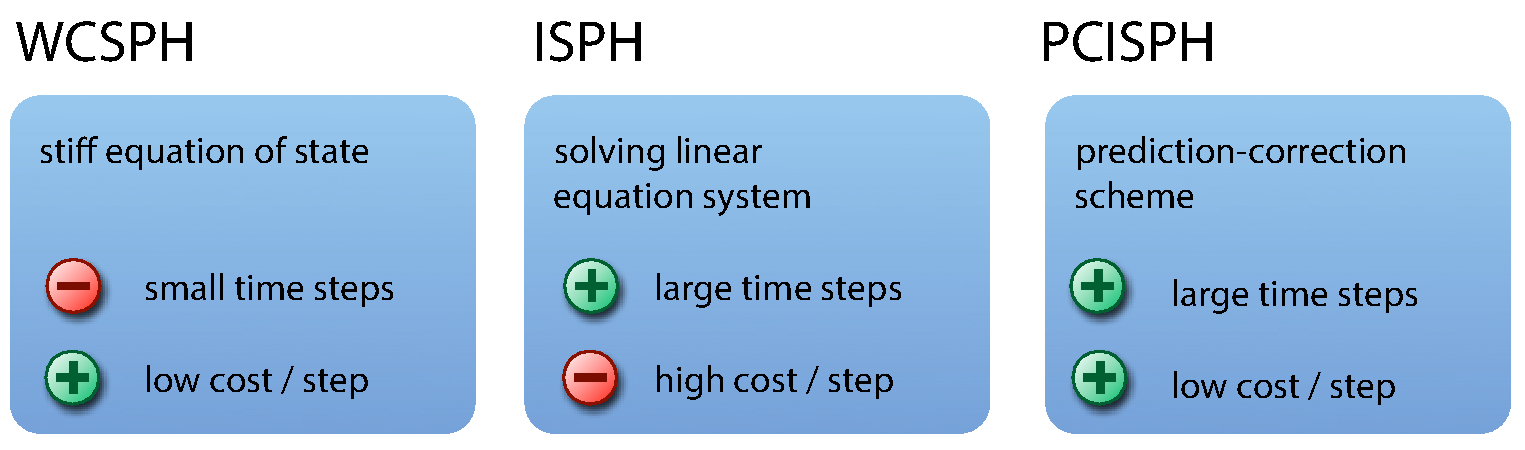
\includegraphics[width=0.45\textwidth]{img/05_incompressibility_methods}
\end{figure}
\begin{description}
	\item[WCSPH] The computation cost increases with decreasing compressibility since the higher stiffness requires smaller time steps.
	\item[ISPH] A possion equation is used to project velocity onto a divergence-free space. The formulation and solving of the equation system is difficult on a unstructured particle configuration.
	\item[PCISPH] The pressure is updated efficiently by an iterative prediction-correction scheme.
\end{description}

%\begin{figure}[H]
%	\centering
%	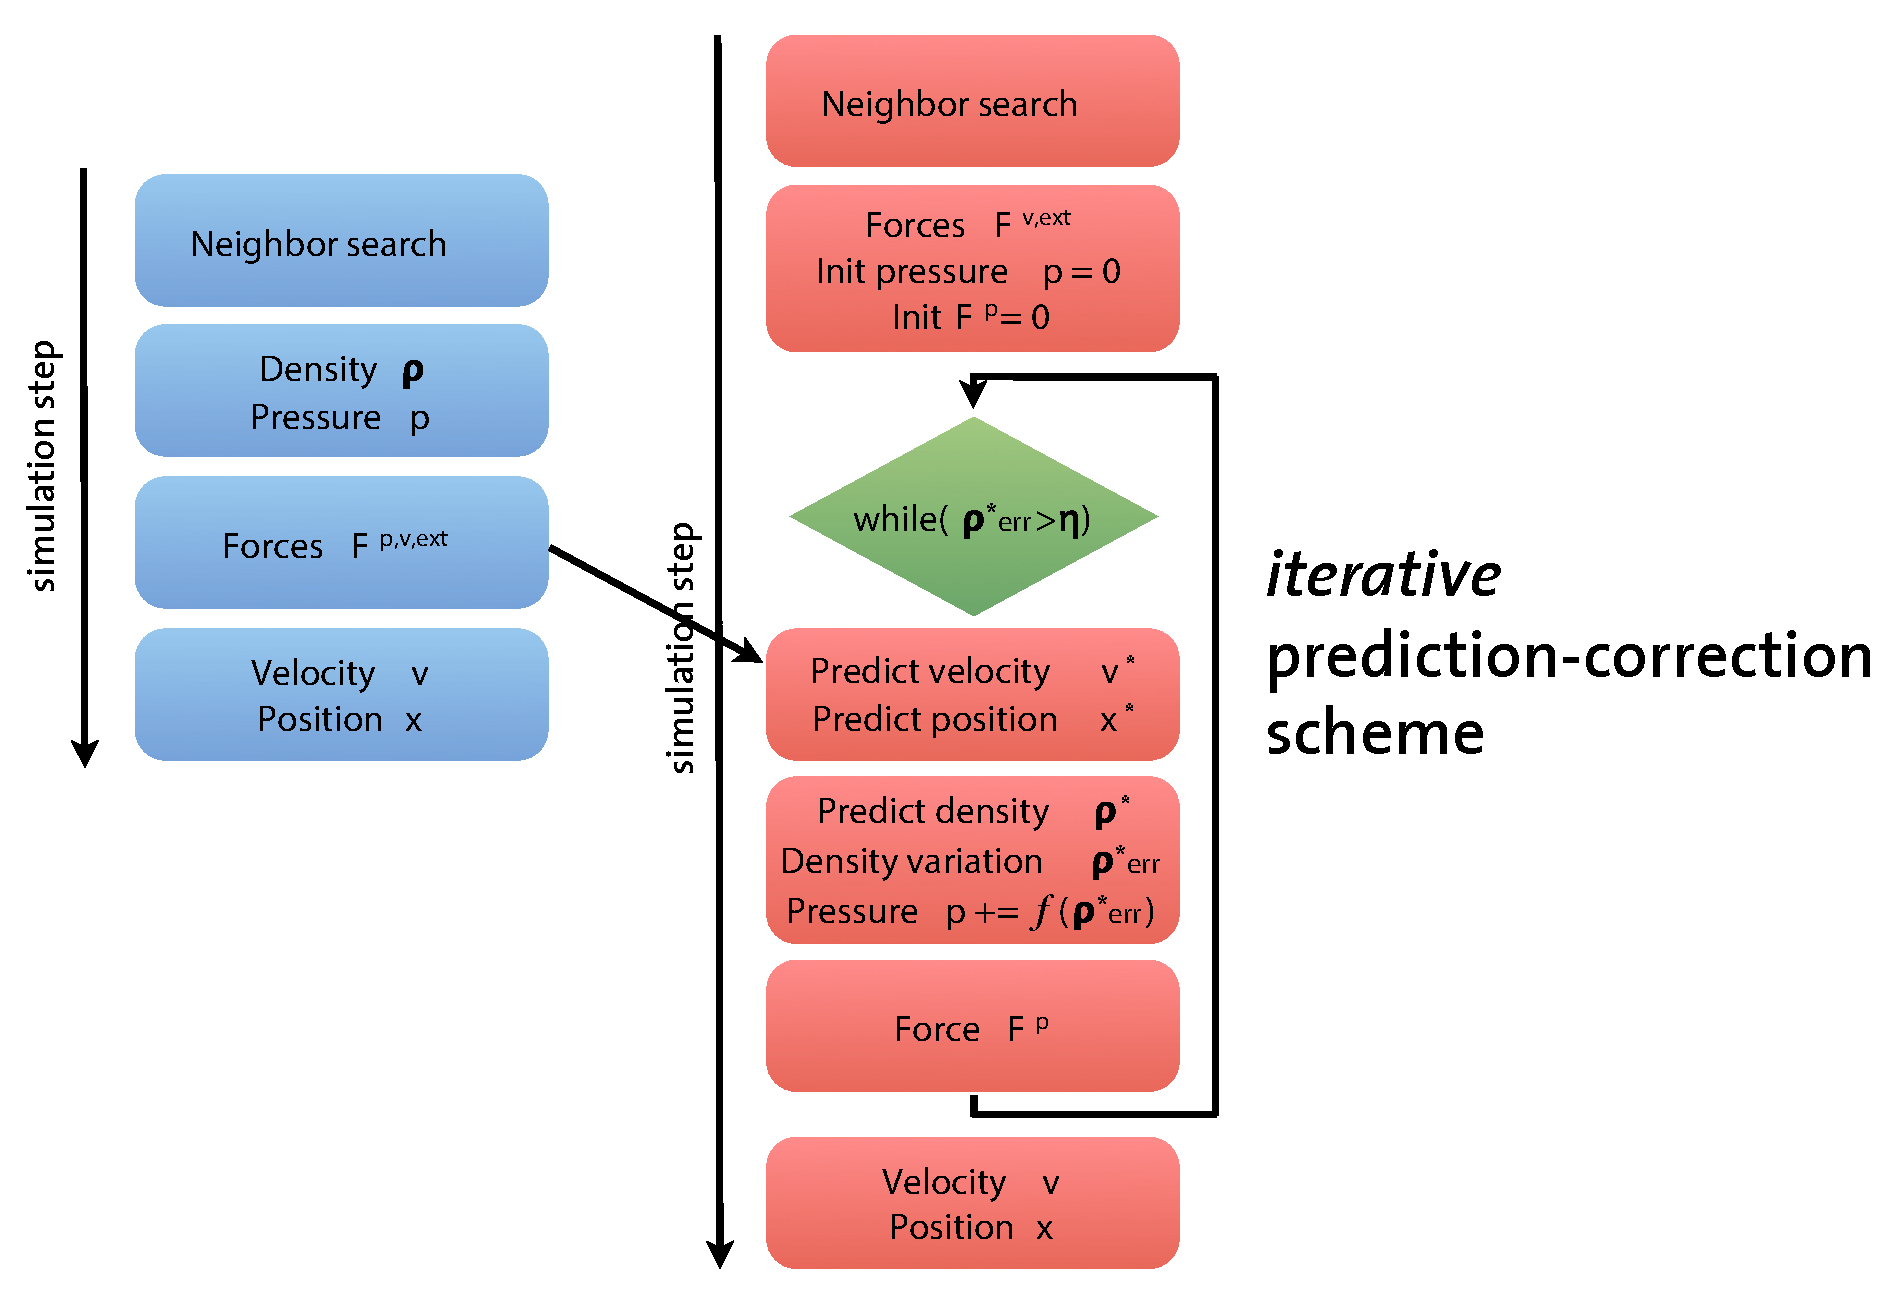
\includegraphics[width=0.45\textwidth]{img/05_pcisph}
%	\caption{PCISPH}
%\end{figure}
%
%\section{Shallow Water Equations (SWE)}
%The Shallow Water Equations are based on the Navier-Stokes Equations:
%\begin{align*}
%	{Dh\over Dt} &= -h \nabla u\\
%	{Du\over Dt} &= -g \nabla(h+H) + a_{ext}
%\end{align*}
%
%Velocity is usually represented as the change of column height per time.
%\begin{figure}[H]
%	\centering
%	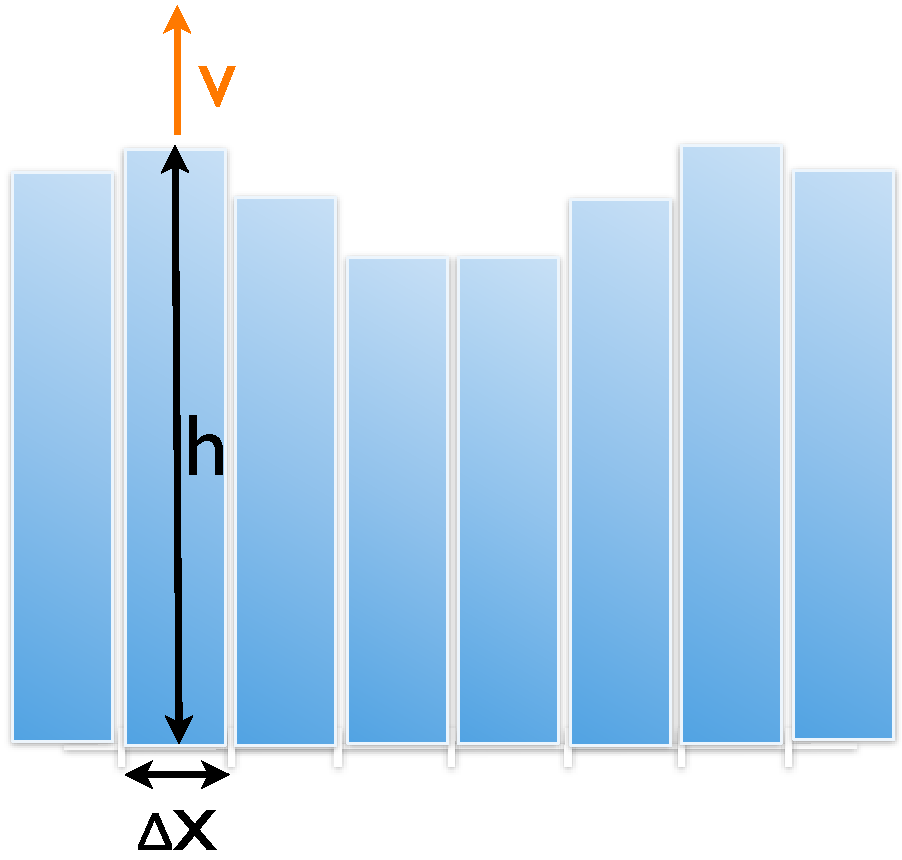
\includegraphics[width=0.35\textwidth]{img/05_swe_overview}
%\end{figure}
%SWE works well for local phenomena like puddles or waves around a boat. Since SWE work only with a vertical velocity field, effects such as whirlpools and the flow of a river cannot be treated correctly. 


 


\end{multicols}